%!TEX root = tesi.tex
\chapter{Results}\label{ch:results}

In this chapter we evaluate the path prediction system; first we describe how our system can emulate OSPF by analyzing the results of the model training; finally we discuss the performance of the path prediction model as a substitute to more traditional routing algorithms. For a more complete analysis, we also implement the same Deep Neural Network (DNN) described in \cite{Kato}, a traditional neural network with four hidden layers and sixteen neurons in each layer. We use this network to compare the performance between DNNs and LSTM for the same task and understand if our hypothesis about RNNs is correct.

\section{Learning from OSPF}
Our system is built to learn the  behavior of OSPF across different configurations, and correlate it with different traffic patterns. We use a LSTM RNN as a learning algorithm and build a model for each source-destination pair in our topology (Figure~\ref{fig:topology}): the total number of models is given by all the possible source-destination  pairs, with the destination addresses considered only on the outer routers not considering the source; for any given a router, the number of addresses associated to it is equal to the number of its interfaces. In our considered scenario, this resulted into a set of $162$ distinct models that are used to determine the hop-by-hop path from a source router to a specific destination address. The path is computed iteratively as follows: starting from the source, the model for the selected destination is used to predict the next hop, then the predicted next hop becomes the new source router; the process is then repeated until the predicted hop is the final destination. Given their significant size, it is unfeasible to analyze all models individually; we are interested in exploring the overall performance. To do so, we analyze the average accuracy and loss over all different models, as discussed in the previous chapter.

Figure~\ref{fig:training_avg} shows the model training progress over time in terms of accuracy and loss: the plot shows the average of the metrics over all $162$ models. The slopes of the graphs give us an idea of what is happening during the training phase: at the beginning (epochs 0-20), both slopes are very steep, indicating that the model is abandoning the initial randomness and converging towards a final stable solution. Afterwards, from epoch 20 to 60, as the gradient diminishes, the slope starts to decrease slowly, indicating that the gradient has probably entered the region of the space in which it will converge to the problem solution. Finally, the curve becomes almost flat, showing that the gradient has reached its  minimum. Note how in both graphs, the two curves have the same behavior: this shows that the model is learning ``without losing generalities``. An increasing accuracy on the training set with a steady or decaying validation accuracy would be a clear sign of overfitting, a situation in which the model becomes too specialized on the training data and it is not able to properly classify new samples. 
The figure shows better performance for both accuracy and loss on the validation data rather than on the train data; even if generally unusual, the reasons of this behavior can be found in the dropout regularization technique. At training time, because of dropout, only part of the network is used; on the other hand, when testing the development of the model on the validation set, regularization mechanisms (i.e., dropout) are turned off, so the network is used in its completeness. This means that the whole network is used to measure accuracy and loss on the validation set but only a part of it is used for the same metrics at training time: for this reason, the performance on the validation set are slightly better than on the training set. 


\begin{figure}
\centering
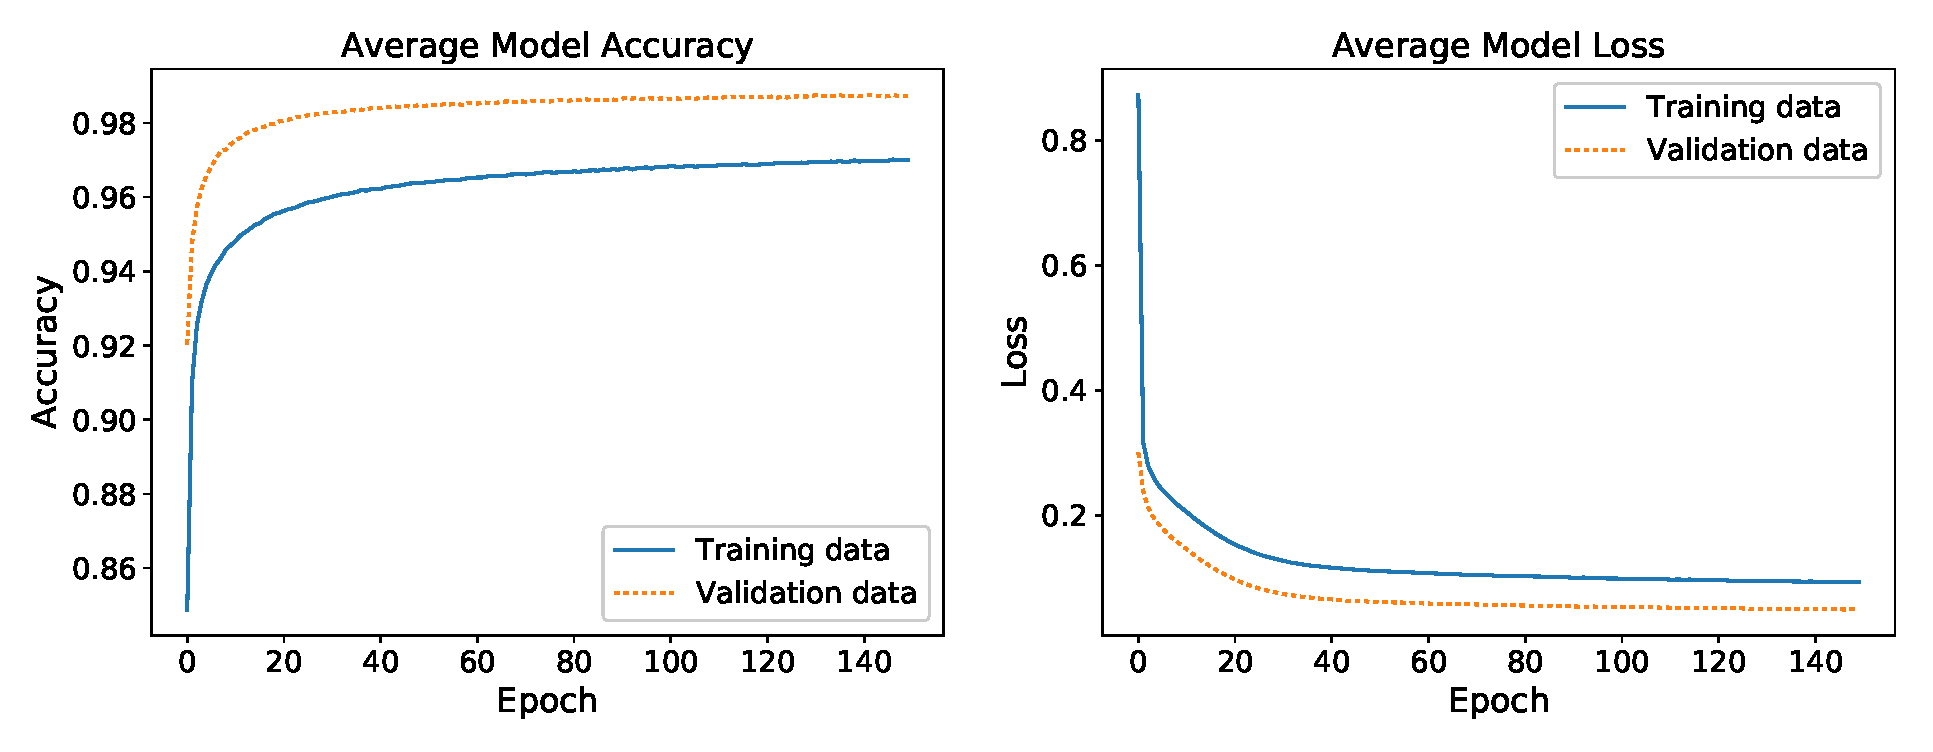
\includegraphics[width=\textwidth]{img/avg_training_metrics}
\caption{Training accuracy and loss progress on training and validation data.}
\label{fig:training_avg}
\end{figure}

To understand how well our model can emulate OSPF we need to analyze the performance on the test set; as we did for the training, we evaluate the performance of the system by averaging the results of the single models. The system achieves an average accuracy of $\textbf{98.71\%}$, with a loss of only $\textbf{0.0496}$; showing really promising results. 
%
With an accuracy of almost $99\%$, LSTM-RNNs performs better than traditional DNNs~\cite{Kato}, which achieves around 90\% of accuracy; however this comparison should be taken with caution, considered that the topologies in the two experiments are slightly different and experiments reproducibility is an open issue in machine learning~\cite{olorisade2017reproducibility}. The comparison of these two approaches is shown in Figure~\ref{fig:lstm_dnn}.

\begin{figure}[b]
\centering
\includegraphics[width=\textwidth]{img/lstm_dnn}
\caption{LSTM and DNN performance comparison.}
\label{fig:lstm_dnn}
\end{figure}

It is important to notice that in this case, the average accuracy could be slightly misleading: the models that represent our model --- a source-destination pair connected by a single link --- are oversimplified, hence it is very likely for them to have an accuracy close to $100\%$. Nonetheless, only $32\%$ (obtained counting all directly connected targets including all the interfaces on the destination router) of the models represents this situation, that means that even if they all had $100\%$ accuracy, the remaining models would have an average accuracy of $97.89\%$.

\section{Overwriting OSPF Routing}
To evaluate our model as OSPF substitution, we observe the behavior of the path prediction system in a functioning network. 
In particular, we  use the same topology (Figure~\ref{fig:topology}) and traffic simulator adopted in the dataset generation phase; to ease the analysis process, all links are set to the same rate. Afterwards, we select a source router and a destination address and examine the difference in behavior between OSPF and our system.

In general, our system shows a dynamic behavior, predicting several paths for the same destination in different traffic conditions. More specifically, we run four traffic simulations, each of them for fifteen minutes, with a varying loss rate on the link chosen by OSPF to connect source and destination;  at the same time, the path prediction system computes a new path every five seconds. The selected target is $(R1, R3)$, with the default path being $R1,R2,R3$ and the loss being varied on the link between R1 and R2. Figure~\ref{fig:path_cmp} compares the routing decisions made by the system in comparisons: being performance unaware, OSPF always chooses the same path, even when the link has losses. Our system on the contrary, shows the ability of behaving dynamically by proposing four alternative paths.

\begin{figure}
\centering
\includegraphics[width=.97\textwidth]{img/path_comparison}
\caption{Routing policies comparison.}
\label{fig:path_cmp}
\end{figure}
By studying the system behavior in presence of losses, it is possible to understand if our model is able to detect and overcome these problems. We test loss rates of 0\%, 5\%,10\%, 15\% and count the number of predictions different from OSPF (table~\ref{tab:same_path_rate}). With the loss set to $0\%$, $43\%$ of the time the predicted path is different from OSPF; if the loss is increased to $5\%$, the ratio of path different from OSPF slightly rises to $45\%$, indicating that the system is able to detect the change. The same happens for a loss of $10\%$, with a much more noticeable improvement in the system behavior;  $63.5\%$ of the proposed paths are in fact, different from the one chosen by OSPF. For the successive loss rate, equals to $15\%$, the performance goes down a little with only a $59.5\%$ different path ratio; the reasons for this loss in performance are discussed in chapter~\ref{ch:conclusion}. The ideal behavior would be for the system to detect the link loss and consequently stop predicting paths going through the damaged link. In our analysis this happens only with a limited loss rate.


Table~\ref{tab:retransmission_rate} compares the resulting retransmission rate of our system, OSPF and Equal Cost Multi Path (ECMP) routing algorithm. The retransmission rate is computed by taking into account how many times traffic would pass through the leaky link, considering two equal-cost paths for ECMP and the ratios in table~\ref{tab:retransmission_rate} for our system. Overall, the system we propose, has a lower retransmission rate than the other strategies, reaching therefore a higher throughput. Figure~\ref{fig:prediction_cmp} is a graphical comparison of the three strategies, showing the time difference needed to transmit the same amount of data. If there is no loss, the three approaches behave the same, however, as soon as a loss rate is introduced, the gap between the curves increases. This increases with the loss rate; however, while it is evident with respect to OSPF, the variation between ECMP and our system is less pronounced.

\begin{table}
\centering
{%
\begin{tabular}{|c|c|c|}
\hline
\multicolumn{1}{|l|}{\textbf{Link loss}} & \multicolumn{1}{l|}{\textbf{Different path rate}} & \multicolumn{1}{l|}{\textbf{Same OSPF path rate}} \\ \hline
0\% & 43\% & 57\% \\ \hline
5\% &45\% & 55\% \\ \hline
10\% & 63.5\% & 36.5\% \\ \hline
15\% & 59.5\% & 40.5\% \\ \hline
\end{tabular}%
}
\caption{Path predictions different and equal to OSPF.}
\label{tab:same_path_rate}
\end{table}

\begin{table}
\centering
\begin{tabular}{|c|c|c|c|c|}
\hline
\multicolumn{1}{|l|}{}  & \multicolumn{4}{c|}{\textbf{Routing Strategy}}                                          \\ \hline
\textbf{Link loss rate} & \textbf{OSPF} & \textbf{ECMP} & \textbf{DNN} &\textbf{LSTM} \\
\hline
0\% & 0\% & 0\% & 0\% & \textbf{0\%}\\
\hline
5\%  & 5\% & \textbf{2.50\%} & 2.70\%	 &2.75\%\\
\hline
10\% & 10\% & 5\% & 7.70\% & \textbf{3.65\%}\\
\hline
15\% & 15\% & 7.50\% & 9\% &\textbf{6.07\%}\\
\hline
\end{tabular}%
\caption{Routing strategies retransmission rate comparison.}
\label{tab:retransmission_rate}
\end{table}

\begin{figure}
\centering
\includegraphics[width=\textwidth]{img/prediction_full_cmp_bar}
\caption{Routing policies retransmission comparison.}
\label{fig:prediction_cmp}
\end{figure}
There is another consideration that needs to be made when talking about OSPF. It would be unfair to consider this protocol completely performance unaware; during our tests, we have noticed that starting from a certain point, OSPF is  able to detect the problem. In our case, with a link loss greater than or equal to $20\%$, OSPF changes its output, selecting a new shortest path. This behavior is caused by the fact that when the loss on the link is too high, the HELLO (i.e., keep-alive) packets used by the protocol are lost, causing the link discovery part of the algorithm to deviate to other routes. We believe that this is a Mininet's limitation and its way to interpret the loss as a fixed phenomenon happening on the link. We know that in real networks losses don't work this way, therefore we are limited in the testing possibilities; nonetheless these results look promising.

\section{A critical scenario}
To have a more clear idea about our system capabilities, we test it in a critical scenario. We decide to simulate a network in which statistically, half of the links are affected by a loss rate; we test the same loss rates of the previous experiments ($5\%$, $10\%$, $15\%$), ten times each, generating traffic between five different targets. The purpose of this experiment is to understand if our system can tolerate better than OSPF a condition where half of the network is not functioning properly. To compare the performance of the two approaches we counted the number of times the links with loss were used; the results are shown in Figure~\ref{fig:stress_test}. The chart compares the total number of defective links traversed in all the runs for each link loss rate. From the results, it appears that our proposed system does not introduce any significant advantage under critical circumstances; the chart shows in fact, that overall, the performance of the two systems are similar, with OSPF performing better when the link loss rate is set to $10\%$ and $15\%$. The reasons of these poor performance are to be found in how our system works: we trained our model to predict alternative paths based on the network conditions; even in this case, the proposed system is able to suggest alternative paths. The main problem is that, given that half of the link in the networks is affected by a loss, the majority of the proposed alternative paths passes through these links, resulting in poor performance. In the conclusions (chapter~\ref{ch:conclusion}) we give a few hints on how to overcome such limitations of our system.

\begin{figure}
\centering
\includegraphics[width=0.949\textwidth]{img/stress_test}
\caption{Comparison of the number of (severely) lossy links traversed by OSPF and LSTM.}
\label{fig:stress_test}
\end{figure}
